\subsection{Separable points}
\label{sec: knnSep}

\begin{figure}
\hfill
\subfigure[Default]{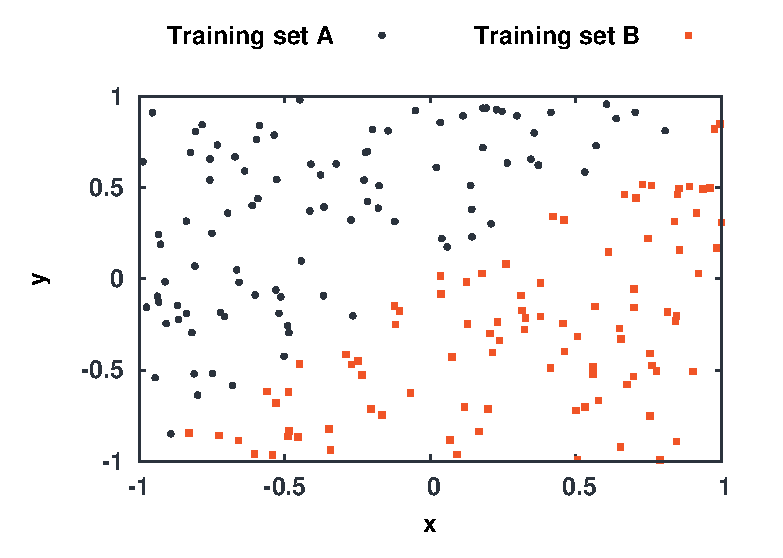
\includegraphics[width=0.48\textwidth]{figures/knn_95_85_separable_default_weighted_samples.eps} \label{fig: knnSepTrainSetDef}}
\hfill
\subfigure[Distant]{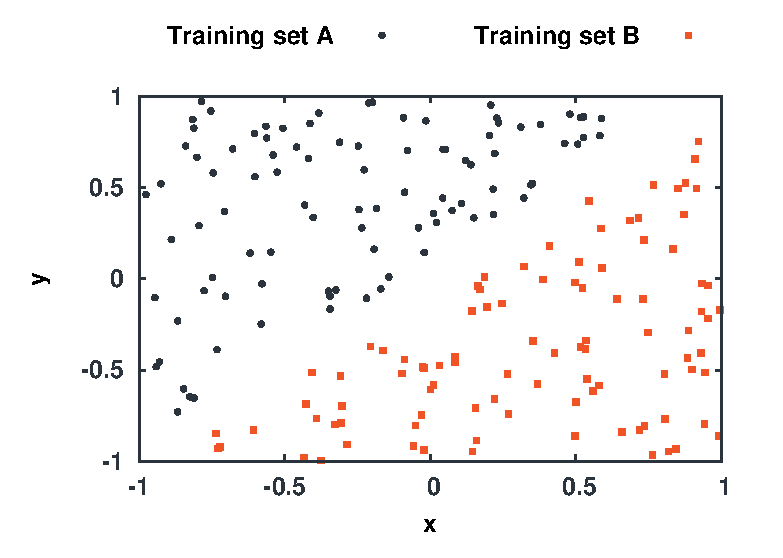
\includegraphics[width=0.48\textwidth]{figures/knn_95_85_separable_distant_weighted_samples.eps} \label{fig: knnSepTrainSetDis}}
\hfill
\centering\subfigure[Overlapped]{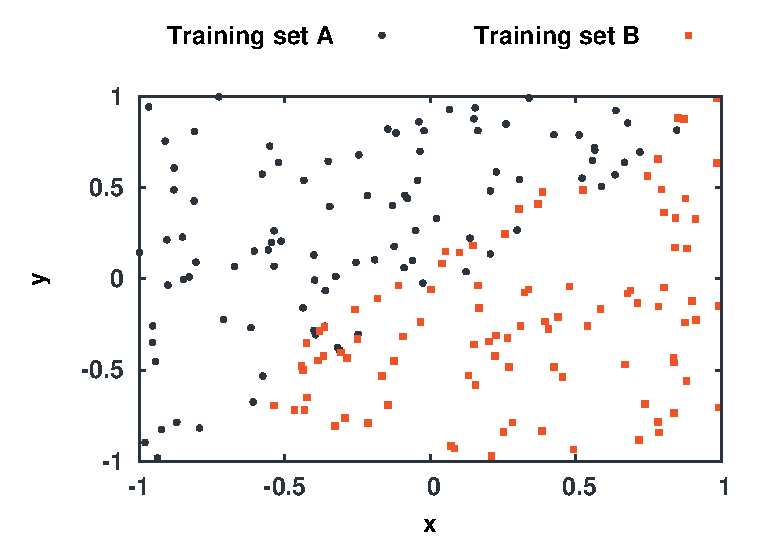
\includegraphics[width=0.48\textwidth]{figures/knn_95_55_separable_overlapped_weighted_samples.eps} \label{fig: knnSepTrainSetOvr}}
\hfill
\caption{Training sets for points separable by $f(x) = x$.}
\label{fig: knnSepTrainSet}
\end{figure}

Lets consider something defined mathematically better than {\it blue} and {\it orange}, i.e. two classes of points which can be separated linearly, e.g. by the line $f(x) = x$ as presented on Fig. \ref{fig: knnSepTrainSet} in three scenarios:

\begin{itemize}
 \item points are exactly separated by $f(x) = x$, Fig. \ref{fig: knnSepTrainSetDef}
 \item there is a small gap to make points more separated, Fig. \ref{fig: knnSepTrainSetDis}
 \item points overlap a little, Fig. \ref{fig: knnSepTrainSetOvr}
\end{itemize}

For each scenario the efficiency of kNN as a function of the size of training sets ($n$) and $k$ is checked in the following way:

\begin{enumerate}
 \item generate $n$ random points above $f(x) = x$ (training set A)
 \item generate $n$ random points below $f(x) = x$ (training set B)
 \item generate a random point
 \item find $k$ nearest neighbors of this point
 \item let them vote:
 \begin{itemize}
  \item with vote weight = $1$ (unweighted)
  \item with vote weight = $1/$distance (weighted)
 \end{itemize}
 \item repeat points 3-5 $N$ times to get good enough statistics ($N = 10^5$ for presented results, but every $100$ test points new training sets are generated)
 \item calculate the score = no. of correctly guessed points / no. of all test points
\end{enumerate}

The efficiency of kNN as a function of $k$ and $n$ can be found on Fig. \ref{fig: knnSepRes}. Clearly, weighted voting gives better results, especially for $k \sim n$. However, even unweighted kNN still gives score better than 90\%. The efficiency is almost the same when extra gap is generated between training sets (Figs. \ref{fig: knnSepResDisU} and \ref{fig: knnSepResDisW}), but it becomes much worse if training sets overlap (Figs. \ref{fig: knnSepResOvrU} and \ref{fig: knnSepResOvrW}).

\begin{figure}
\hfill
\subfigure[Default, unweighted]{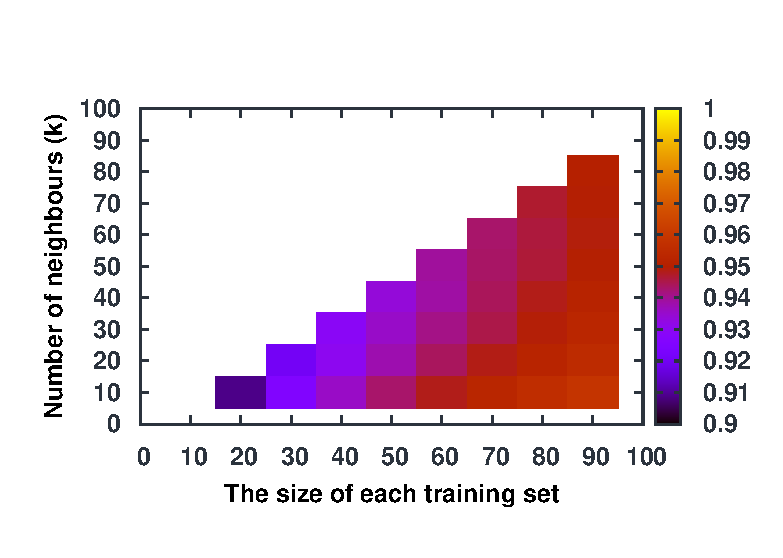
\includegraphics[width=0.48\textwidth]{figures/knn_separable_default_unweighted.eps} \label{fig: knnSepResDefU}}
\hfill
\subfigure[Default, weighted]{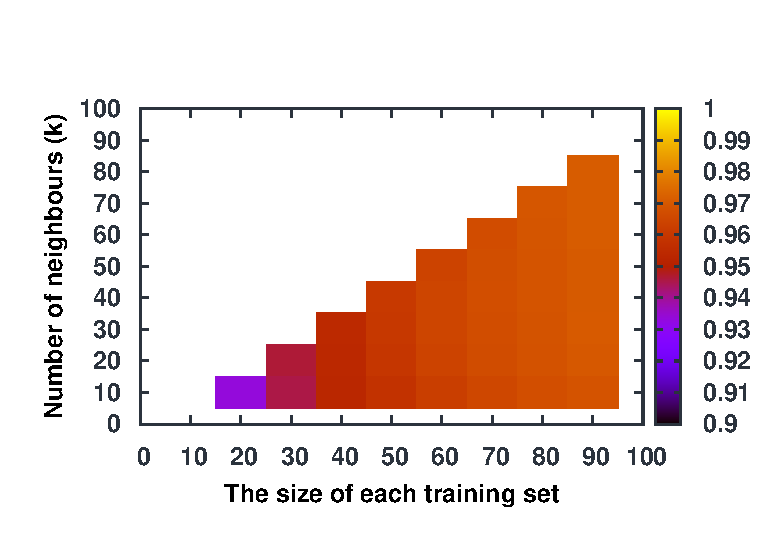
\includegraphics[width=0.48\textwidth]{figures/knn_separable_default_weighted.eps} \label{fig: knnSepResDefW}}
\hfill
\subfigure[Distant, unweighted]{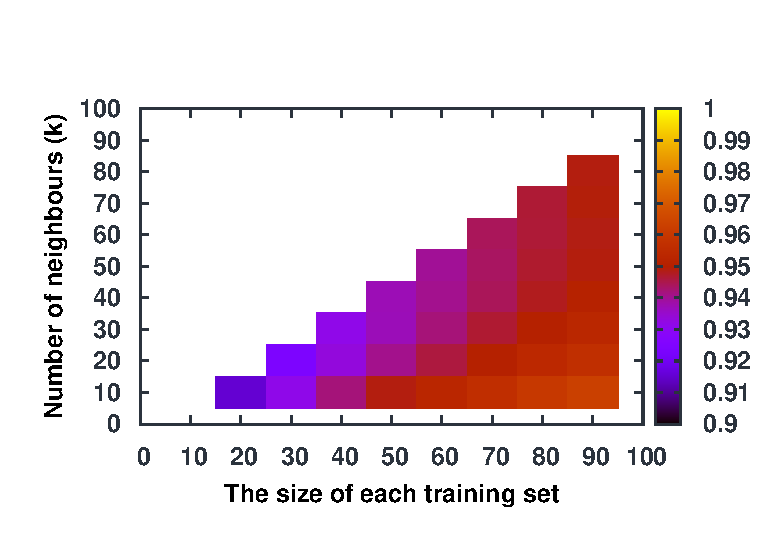
\includegraphics[width=0.48\textwidth]{figures/knn_separable_distant_unweighted.eps} \label{fig: knnSepResDisU}}
\hfill
\subfigure[Distant, weighted]{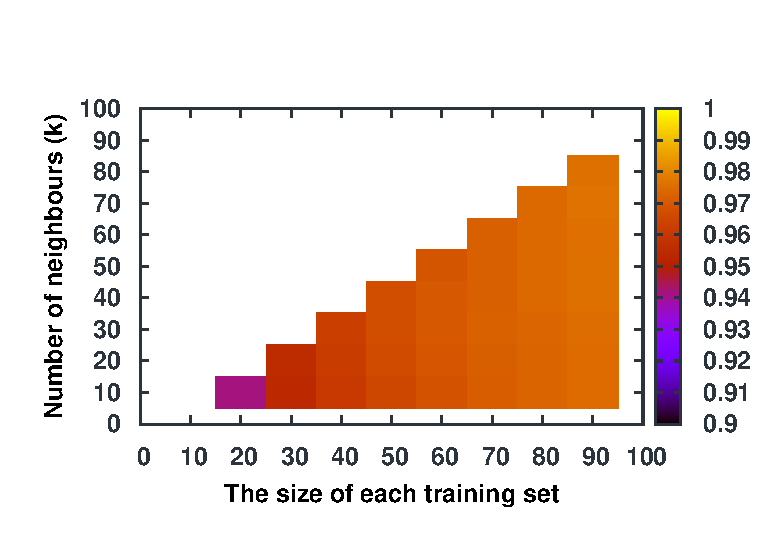
\includegraphics[width=0.48\textwidth]{figures/knn_separable_distant_weighted.eps} \label{fig: knnSepResDisW}}
\hfill
\subfigure[Overlapped, unweighted]{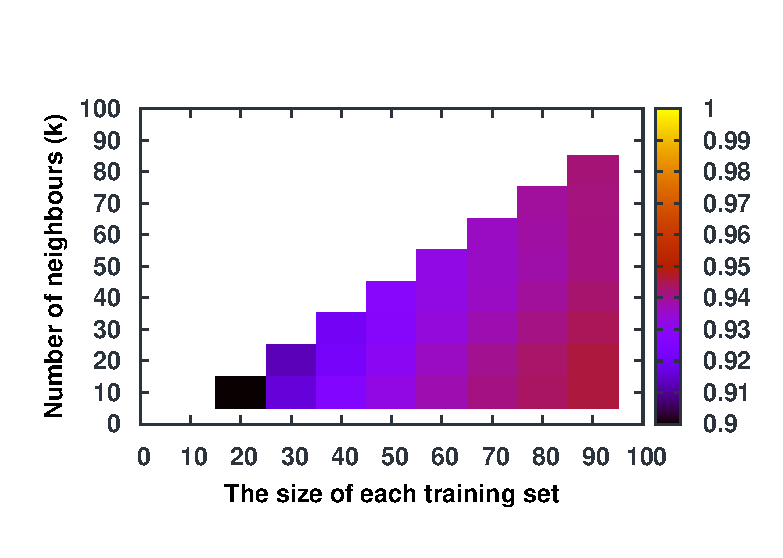
\includegraphics[width=0.48\textwidth]{figures/knn_separable_overlapped_unweighted.eps} \label{fig: knnSepResOvrU}}
\hfill
\subfigure[Overlapped, weighted]{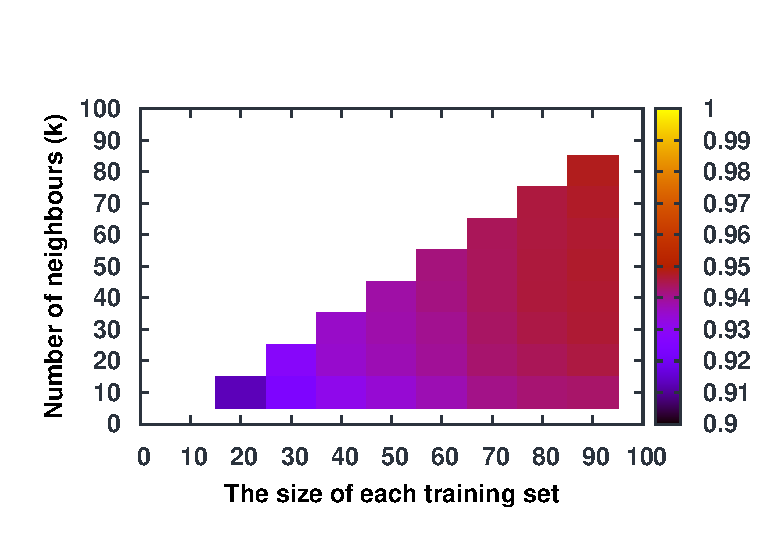
\includegraphics[width=0.48\textwidth]{figures/knn_separable_overlapped_weighted.eps} \label{fig: knnSepResOvrW}}
\hfill
\caption{kNN efficiency for points separable by $f(x) = x$.}
\label{fig: knnSepRes}
\end{figure}

\begin{figure}
\hfill
\subfigure[Training sets]{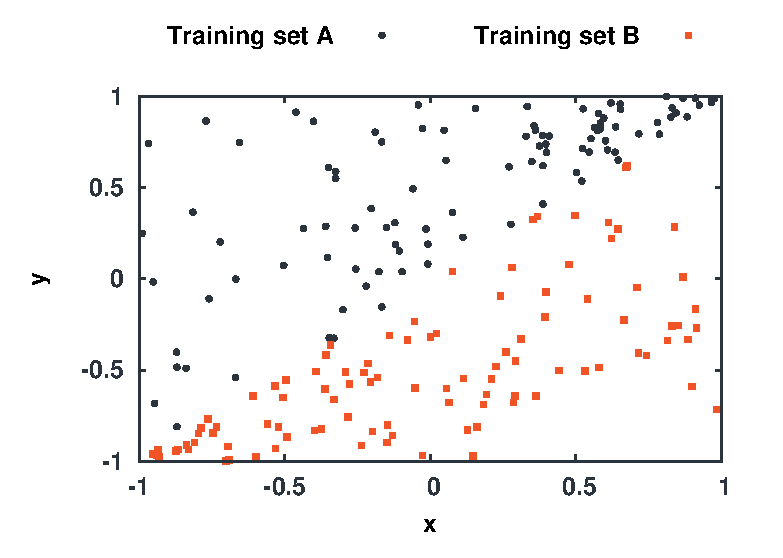
\includegraphics[width=0.48\textwidth]{figures/knnWrongTrainSet.eps} \label{fig: knnWrongTrainSet}}
\hfill
\subfigure[Testing set]{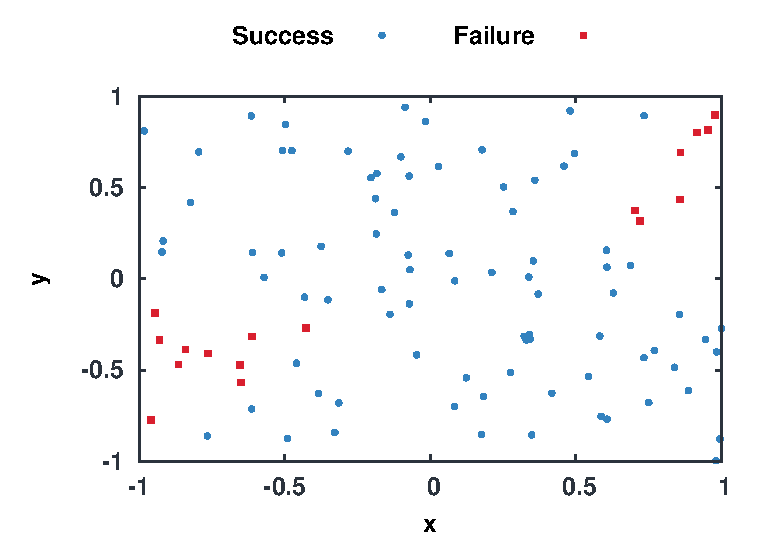
\includegraphics[width=0.48\textwidth]{figures/knnWrongTrainResults.eps} \label{fig: knnWrongTrainResults}}
\hfill
\hfill
\caption{The example of the kNN classification using wrong training sets ($n = 100$, $k = 50$).}
\label{fig: knnWrongTrain}
\end{figure}

Lets take a look what happens when training sets are not uniformly distributed, as presented on Fig. \ref{fig: knnWrongTrain}. It still looks (by eye) that training sets are separated by $f(x) = x$, see Fig. \ref{fig: knnWrongTrainSet}. However, from obvious reasons some points are going to be incorrectly classified, as presented on Fig. \ref{fig: knnWrongTrainResults}.

